\documentclass[preprint,10pt]{elsarticle}

\usepackage{amssymb}
\usepackage{amsmath}
\usepackage{lineno}
\usepackage{hyperref}

\usepackage{epstopdf}
\usepackage{epsfig}
\usepackage{setspace}

\newcommand{\be}{\begin{equation}}
\newcommand{\ee}{\end{equation}}
\newcommand{\beq}{\begin{eqnarray}}
\newcommand{\eeq}{\end{eqnarray}}
\newcommand{\ba}{\begin{eqnarray}}
\newcommand{\ea}{\end{eqnarray}}

\newcommand{\ua}{{\bf u}_\alpha}
\newcommand{\utwo}{\overline{\bf u}_2}
\setcounter{MaxMatrixCols}{24}

\journal{Coastal Engineering}

\begin{document}


%\title{Model derivations}

\begin{center}
{\bf \Huge Coupling BC plus internal wavemaker}
 \end{center}

I added tests for the coupling application in  the GITHUB repository: 

TMA\_MAKER/TEST\_couplingbc\_wavemaker/

 1) \href{https://github.com/fengyanshi/TMA_MAKER/tree/master/TEST_couplingbc_wavemaker}{Coupling Cases}
 
 2)  \href{https://github.com/fengyanshi/TMA_MAKER/tree/master/TEST_couplingbc_wavemaker/preprocessing}{Preprocessing}

3)  \href{https://github.com/fengyanshi/TMA_MAKER/tree/master/TEST_couplingbc_wavemaker/preprocessing}{Postprocessing}

Four cases are provided for this specific application. The best solution so far involves using (u,v) coupling boundary conditions at the lateral boundaries (south and north) and adding a wavemaker and sponge layer offshore (Cases 3 and 4). Adding tidal elevation is challenging because the sponge layer disrupts the conditions. A new development may be needed to use full hydrodynamic boundary conditions derived from a large-domain model. 

\newpage
\section*{CASE 1: Constant slope with constant v at lateral boundaries}

The computational domain 200m long (East-West) and 100m wide (South-North). The slope start from $x=0$  with slope of 0.055, so that there are dry points at the east boundary (see Figure \ref{v1} top pannel).  A constant velocity $v=1 m/s$ is specified at the south and north boundaries. The coupling file can be generated using /preprocessing/A1\_A\_B.m.  Set $southfine(ipoint,2,ti)=1.0$ and $northfine(ipoint,2,ti)=1.0$. 

The test is used to examine the x-distribution of $v$ inside the domain. Because the water depth decreases on shore, the smaller $v$ velocity is expected in shallower water depth (refer to the theory of open channel flow). The second panel in Figure \ref{v1} shows the $v$-distribution along $x$ at  $y = 50m$ (middle). The spatial distribution of $v$ is shown in the third panel. The bottom pattern shows the vertical vorticity, indicating strong shear at the shoreline. 
  
    
 \begin{figure}
\begin{center}
 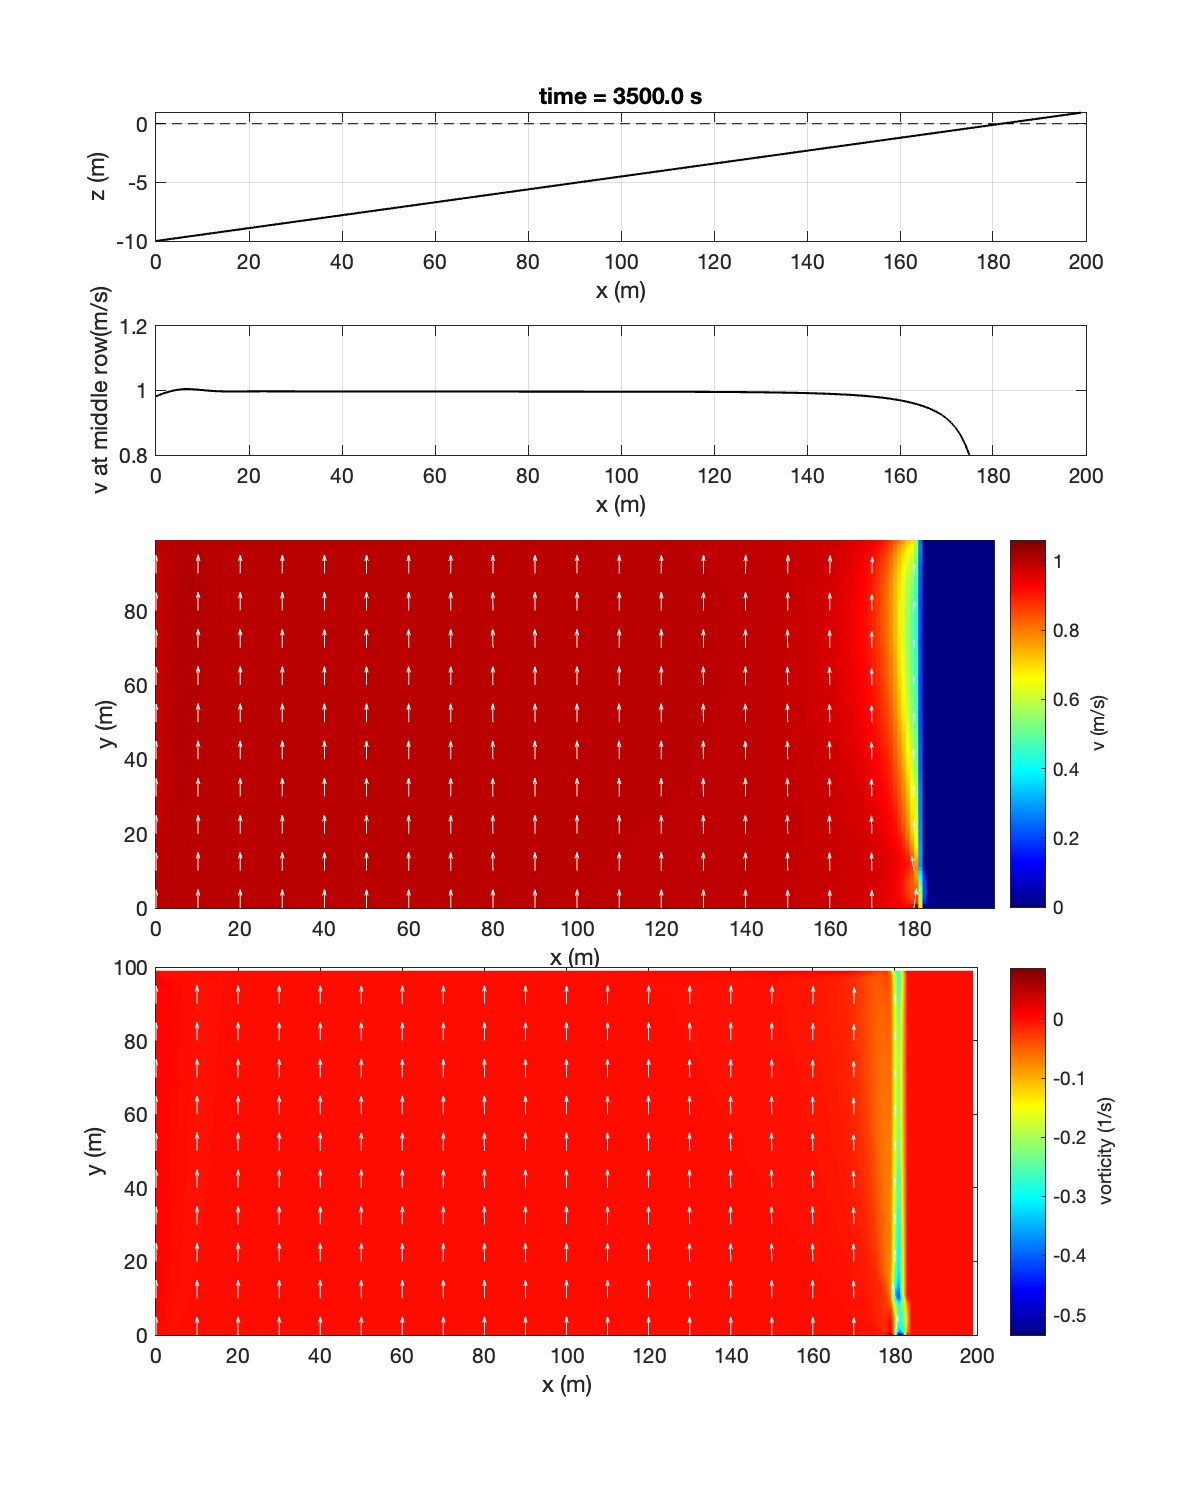
\includegraphics[width=0.7\textwidth]{../TEST_couplingbc_wavemaker/postprocessing/case_slope_055.jpg}
 \caption{CASE 1: Constant slope with constant v at lateral boundaries.}
 \label{v1}
 \end{center}
 \end{figure}

\newpage
\section*{CASE 2: Constant slope with varying constant v at lateral boundaries}

The same as CASE 1, except a linear distribution of $v$ from $1 m/s$ to $0$ across-shore. Use the same matlab file and set 
$southfine(ipoint,2,ti)=1.0*(npoints(3)-ipoint)/(npoints(3)-1);$ $northfine(ipoint,2,ti)=1.0*(npoints(4)-ipoint)/(npoints(4)-1);$ 
to generate coupling.txt. The second panel shows $v$ cross-shore distribution at  $y = 50m$ (middle). Note that $v=0$ at all dry points. Compare Case 1, strong shear is only shown at very narrow area (bottom panel) due to the small $v$ near the shoreline. 

\begin{figure}
\begin{center}
 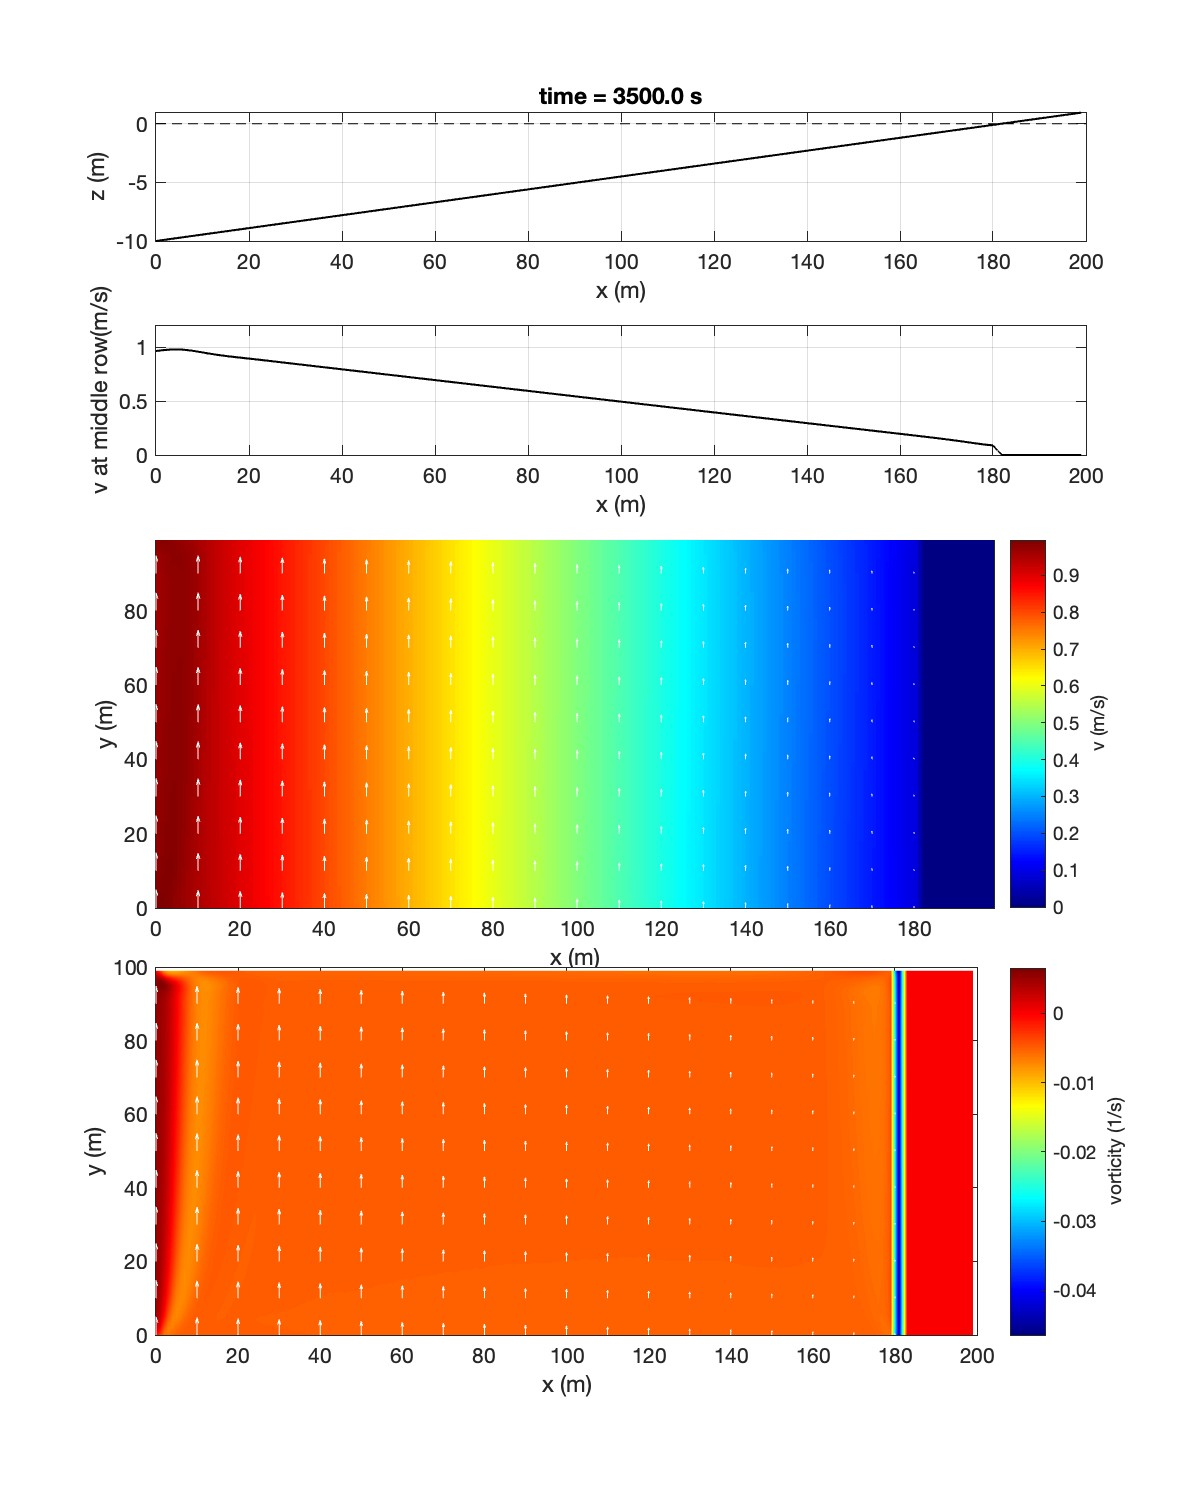
\includegraphics[width=0.7\textwidth]{../TEST_couplingbc_wavemaker/postprocessing/case_slope_055_reduced_v.jpg}
 \caption{CASE 2: Constant slope with varying constant v at lateral boundaries.}
 \label{v2}
 \end{center}
 \end{figure}
  
  \newpage
\section*{CASE 3:Add a wavemaker}
  
  \begin{figure}
\begin{center}
 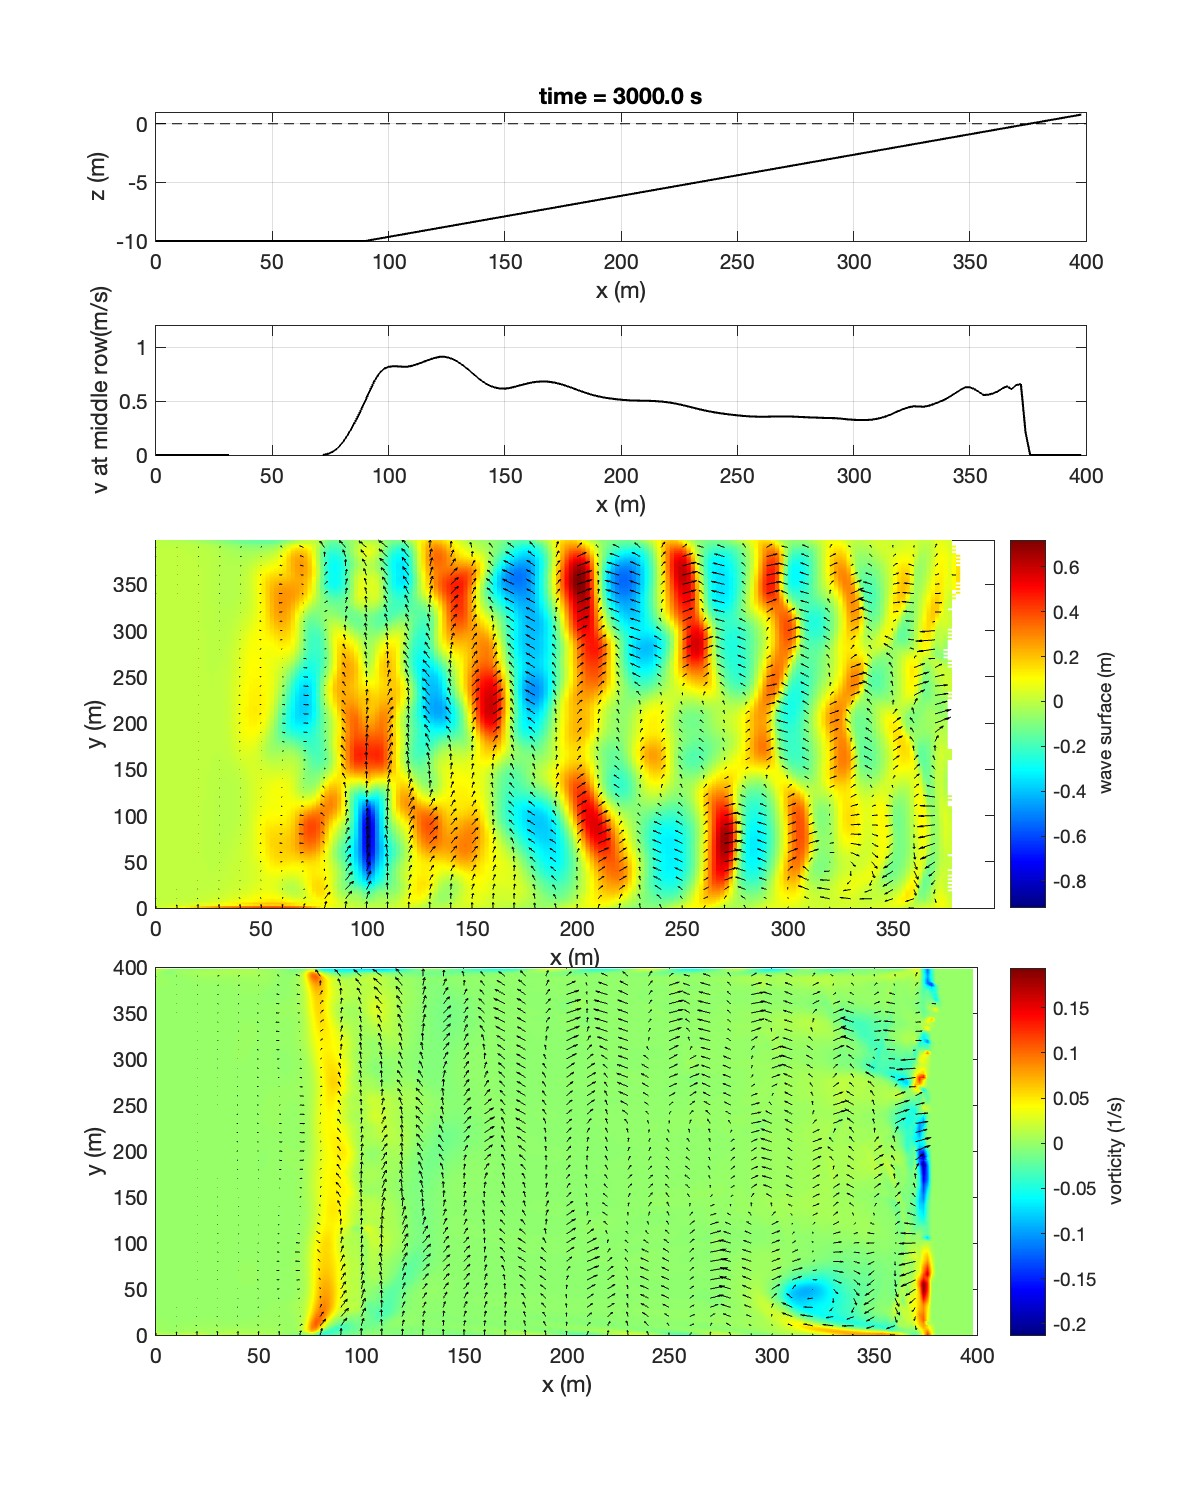
\includegraphics[width=0.6\textwidth]{../TEST_couplingbc_wavemaker/postprocessing/case_slope_wave.jpg}
 \caption{CASE 3: Constant slope with varying constant v at lateral boundaries, plus a wavemaker}
 \label{v2}
 \end{center}
 \end{figure}
 
 Based on Case 1 or Case 2, we can adda wavemake at x=100m, and a sponge layer at the west boundary
 
 \noindent
 WAVEMAKER = WK\_IRR \\
DEP\_WK = 10.0  \\
Xc\_WK = 100.0  \\
Yc\_WK = 200.0  \\
Ywidth\_WK = 390.0 \\
FreqPeak = 0.125  \\
FreqMin = 0.05 \\
FreqMax = 0.3  \\
Hmo = 1.0  \\
GammaTMA = 5.0 \\ 
ThetaPeak = 15.0  \\
Sigma\_Theta = 10.0  \\
 
 \noindent
Sponge\_west\_width =  80.0  
 NOTE: the width of the wavemaker needs to be specified smaller than domain width. Ywidth\_WK = 390.0 
 
 \newpage
 
   \newpage
\section*{CASE 4: Oblique incidence}
 
  \begin{figure}
\begin{center}
 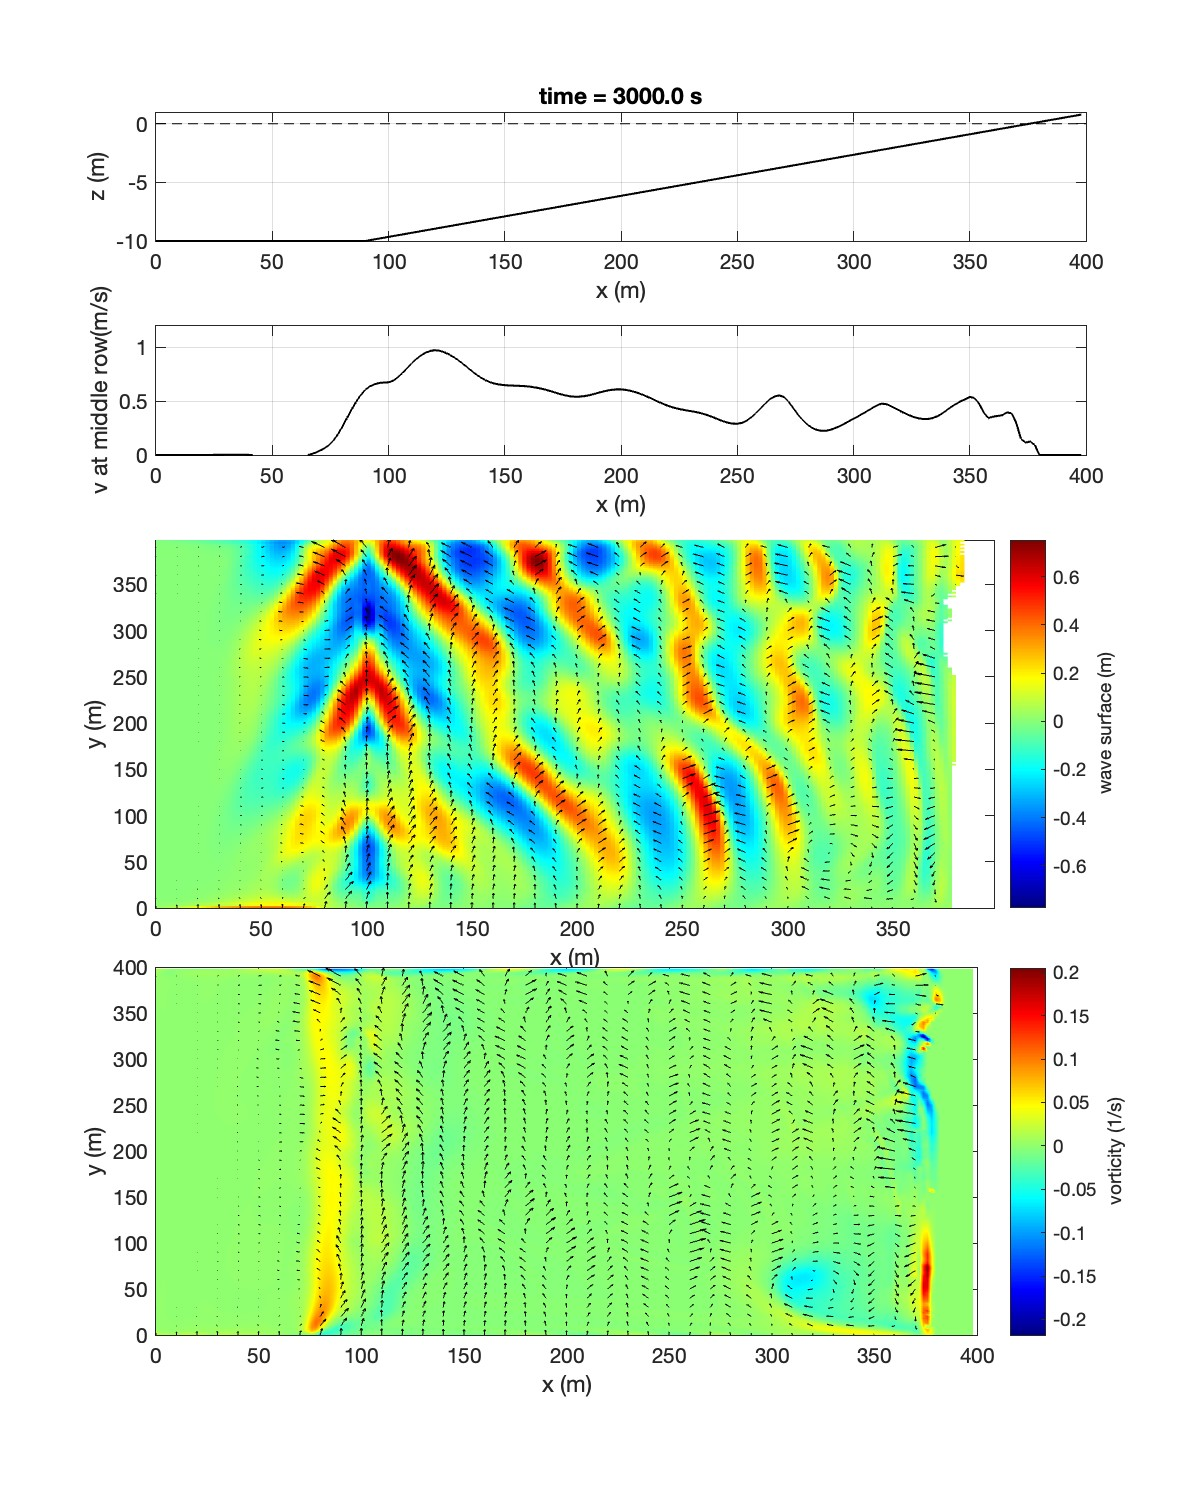
\includegraphics[width=0.7\textwidth]{../TEST_couplingbc_wavemaker/postprocessing/case_slope_wave_15deg.jpg}
 \caption{CASE 4: oblique incidence}
 \label{v2}
 \end{center}
 \end{figure}

Base on CASE 3, modify 

ThetaPeak = 15.0  

You should see wave diffraction at the southern boundary and reflection from the northern boundary. It's hard to avoid!
  
\end{document}







